% POSTER (poster.tex)
\documentclass[a0paper,portrait]{tikzposter}
\usepackage{fontspec}
\usepackage{polyglossia}
\setmainlanguage{russian}
\setotherlanguage{english}
\newfontfamily\cyrillicfont{Times New Roman}

\title{Прыгающий робот с Wi-Fi управлением}
\author{Балдин Виктор, Румянцев Иван, Голицын Артур}
\date{\today}
\institute{МФТИ}

\begin{document}
\maketitle

\block{Цель проекта}{
Создание компактного робота с:
\begin{itemize}
\item Дистанционным управлением через Wi-Fi
\item Автономным питанием
\item Механизмом направленного прыжка
\end{itemize}
}

\begin{columns}
\column{0.5}
\block{Компоненты системы}{
\begin{itemize}
\item Контроллер ESP32
\item Силовые сервоприводы
\item Аккумуляторная батарея
\item 3D-печатный корпус
\end{itemize}
}

\column{0.5}
\block{Характеристики}{
\begin{itemize}
\item Вес: 250 г
\item Высота прыжка: 20 см
\item Радиус действия: 50 м
\item Время зарядки: 2 ч
\end{itemize}
}
\end{columns}

\block{Этапы разработки}{
\begin{tikzfigure}[Схема работы системы]
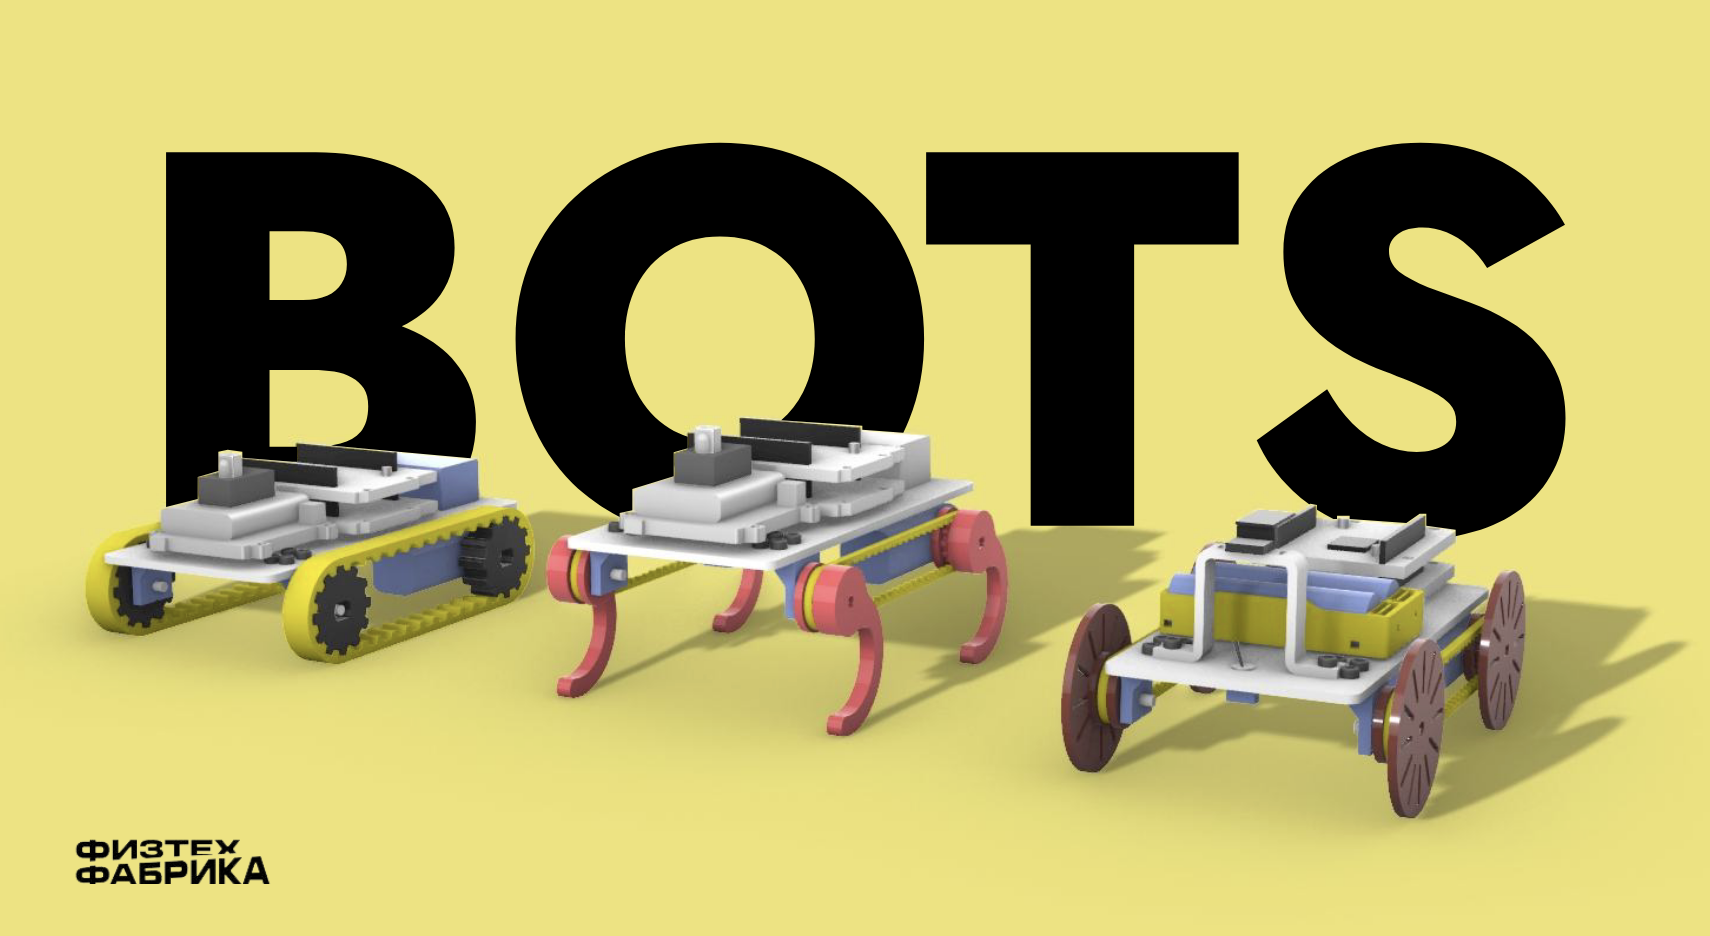
\includegraphics[width=0.3\textwidth]{system_diagram}
\end{tikzfigure}

\begin{enumerate}
\item Проектирование механизма
\item Программирование контроллера
\item Сборка прототипа
\item Тестирование
\end{enumerate}
}

\block{Результаты}{
\begin{itemize}
\item Успешная демонстрация прыжков
\item Стабильная работа Wi-Fi связи
\item Открытый исходный код
\item Возможность модернизации
\end{itemize}
}

\end{document}
